\subsection{Algorithmus}
\label{bpr:algorithmus}

Nachdem in Kapitel \ref{bpr:vorueberlegungen} bereits die formalen Grundlagen für die Beschreibung des \bpr-Algorithmus geschaffen wurden, können wir nun präziser auf die Funktionsweise des Algorithmus eingehen. Die Basis für das Verfahren bildet die Nutzung von Abhängigkeiten zwischen mehreren Suffixen: Teilen sich zwei Suffixe \suffix{i} und \suffix{j} einen gemeinsamen Präfix der Länge \(\textit{offset}\), so ist zunächst festzustellen, dass \suffix{i+\textit{offset}} bzw. \suffix{j+\textit{offset}} nicht nur Suffixe von \inputtext, sondern auch Suffixe von \suffix{i} bzw. \suffix{j}  sind. Die Reihenfolge von \suffix{i} und \suffix{j} im Suffix-Array kann also einfach durch die Reihenfolge der eventuell bereits zuvor sortierten Suffixe \suffix{i+\textit{offset}} und \suffix{j+\textit{offset}} bestimmt werden. Um allerdings auf eine derartige Vorsortierung zurückgreifen zu können, muss zu Beginn zumindest eine grobe \glqq initiale Sortierung\grqq{} der Suffixe existieren.\par\smallskip
Um dies zu erreichen, verwendet der hier beschriebene Algorithmus zwei Phasen, von denen die erste dazu dient, die Suffixe initial nach gemeinsamen Präfixen der Länge \(d\) zu gruppieren. Auf Basis dieser Gruppierung werden die Suffixe Buckets zugewiesen, sodass sich zwei Suffixe genau dann im gleichen Bucket befinden, wenn sie einen gemeinsamen Präfix der Länge \(d\) besitzen.\par
In der zweiten Phase werden dann die Buckets anhand der oben genannten Vorschrift schrittweise rekursiv verfeinert. Auf diese Weise ergibt sich das fertig sortierte Suffix-Array, sobald jeder Bucket eine minimale Länge von 1 erreicht hat.\par\smallskip
Im Folgenden werden beide Phasen im Detail erklärt. Wir verwenden dafür als Beispiel das Fantasiewort \covfefefe, dessen Suffixe wir mittels \bpr sortieren.

\subsubsection{Erste Phase}
\label{bpr:algorithmus:phase1}

Die erste Phase führt eine Gruppierung der Suffixe nach gemeinsamen Präfixen der Länge \(d\) durch. Die Wahl eines geeigneten Parameters \(d\) wird nicht vom Algorithmus übernommen, es wird allerdings empfohlen, \(d < \log n\) zu wählen \cite{saca:2}.\par
Um nun alle Suffixe von \inputtext in Level-\(d\)-Buckets zu gruppieren, wird zunächst eine Tabelle \bkt der Länge \((|\Sigma| + 1)^d\) mit Einträgen für alle möglichen Präfixe der Länge \(d\) erstellt, wobei jeder Präfix eindeutig durch den zugehörigen Funktionswert von \coded identifiziert werden kann. In einem sequentiellen Durchlauf des Textes \inputtextplus können dann mithilfe der Eigenschaft aus Gleichung \ref{eq:coded} die Kodierungen der vorkommenden Präfixe effizient berechnet werden. In diesem Durchlauf kann für jeden Präfix \(p\) die zugehörige Anzahl der Vorkommen in \inputtextplus (und damit die spätere Größe des Buckets \(b_p\)) bestimmt werden.\par
Da die Sortierung der Buckets durch den Schlüssel \coded gegeben ist, können im Anschluss anhand der nun bekannten Bucketgrößen auch die Positionen aller Buckets im Suffixarray festgelegt werden.
\begin{figure}[ht]
	\vspace{0.2\baselineskip}
	\resizebox{\textwidth}{!}{
		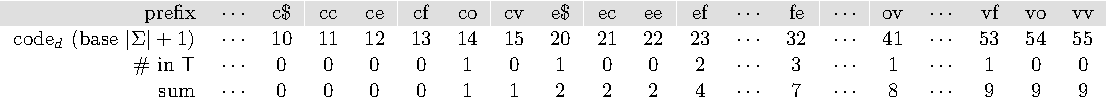
\includegraphics{kapitel/saca_algorithmen/bpr/algorithmus/phase1/bkt/image.pdf}
	}
	\caption[Tabelle \emph{bkt} zur Bestimmung der Bucket-Größen und -Positionen]{Tabelle \emph{bkt} zur Bestimmung der Bucket-Größen und -Positionen. Die Anzahl der Vorkommen eines Präfix im Text ist in Zeile 2 angegeben. Zeile 3 beinhaltet die kumulierte Anzahl und bestimmt damit die linke Grenze des nachfolgenden Buckets.}
	\label{fig:bkt}
\end{figure}
Der entsprechende Stand der Verarbeitung für den Text \(\inputtext = \covfefefe\) ist in Abbildung \ref{fig:bkt} zu sehen. Die kumulierte Größe aller Buckets bis einschließlich Bucket \(j\) legt gleichzeitig die linke Grenze des Buckets \(j+1\) fest. In einem weiteren Durchlauf können jetzt alle Suffixe \(\suffix{0}, \ldots, \suffix{n-1}\) im vorläufigen Suffixarray \sa einsortiert werden. Das Suffixarray beinhaltet dabei für ein Suffix \suffix{i} mit \(0 \leq i < n\) nicht das gesamte Suffix als String, sondern lediglich den Index \(i\) des Suffixes. Abbildung \ref{fig:buckets_initial} zeigt die initiale Einteilung der Buckets für \(d=2\). Zur besseren Visualisierung sind hier in dem Array die Suffixe anstatt der bloßen Indizes angegeben.\par\smallskip
\begin{figure}[ht]
	\resizebox{\textwidth}{!}{
		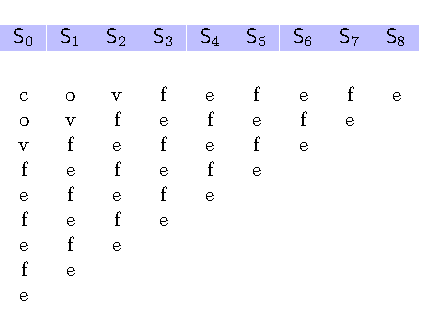
\includegraphics{kapitel/saca_algorithmen/bpr/algorithmus/phase1/sa_initial/image.pdf}
		\hspace{1em}
		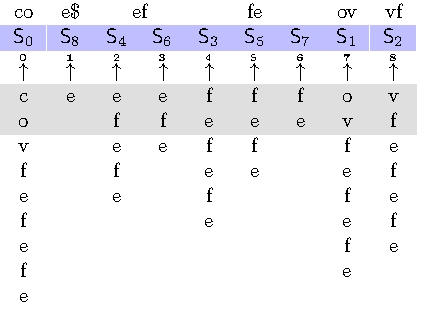
\includegraphics{kapitel/saca_algorithmen/bpr/algorithmus/phase1/buckets_initial/image.pdf}
	}
	\caption[Suffixe unsortiert und nach der ersten Phase des Algorithmus]{Suffixe unsortiert (links) und nach der ersten Phase des Algorithmus (rechts)}
	\label{fig:buckets_initial}
\end{figure}
Wie bereits zuvor erwähnt, wollen wir in der zweiten Phase des Algorithmus die Buckets verfeinern, indem eine weitere Gruppierung jedes bestehenden Buckets aufgebaut wird.\par
\begin{wrapfigure}[15]{r}{0.42\textwidth}
	\vspace{-1em}
	\resizebox{0.42\textwidth}{!}{
		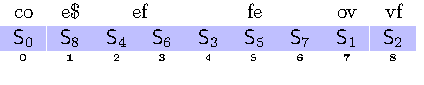
\includegraphics{kapitel/saca_algorithmen/bpr/algorithmus/phase1/buckets_initial_plain/image.pdf}
	}\\
	\resizebox{0.42\textwidth}{!}{
		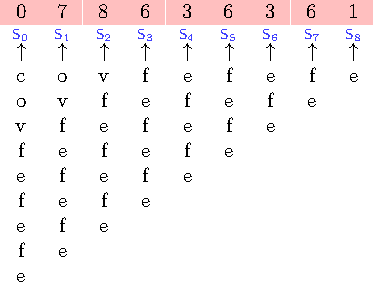
\includegraphics{kapitel/saca_algorithmen/bpr/algorithmus/phase1/bptr_initial/image.pdf}
	}
	\caption[Vorsortierte Suffixe und zugehörige Bucket-Pointer]{Vorsortierte Suffixe und zugehörige Bucket-Pointer}
	\label{fig:bucket_pointer_initial}
\end{wrapfigure}
Wir wollen dazu auf die bereits bekannte Einteilung der Suffixe in Level-\(d\)-Buckets zugreifen und anhand dessen eine weiterführende Sortierung vollziehen. Eine Anfrage, in welchem Bucket sich ein Suffix befindet, ist jedoch mit der bisher eingeführten Datenstruktur nicht effizient zu beantworten. \par
Es wird daher mit dem Bucket Pointer \bptr ein zweites Array eingeführt, welches sinngemäß ein Reverse Mapping des Suffixarrays \sa beinhaltet (s. Abbildung \ref{fig:bucket_pointer_initial}). In diesem Array symbolisiert jeder Index ein Suffix, wobei der Eintrag \(\bptr[i]\) den zugehörigen Bucket angibt, welcher jeweils über seine rechte Grenze identifiziert wird. Die Bestimmung der Grenzen erfolgt durch Ablesen der kumulierten Summe aus der Tabelle \bkt.

\subsubsection{Zweite Phase}
\label{bpr:algorithmus:phase2}

Zu Beginn dieser Phase des Algorithmus existiert bereits ein (noch nicht fertig sortiertes) Suffix-Array \sa, welches nun rekursiv sortiert werden soll. Die aktuelle Einteilung der Suffixe in Buckets ist über den Bucket Pointer \bptr gegeben, aus dem abgelesen werden kann, ob sich zwei Suffixe im gleichen oder in verschiedenen Buckets befinden. Das Array \bkt, welches in der ersten Phase des Algorithmus erstellt wurde, um die initiale Zuteilung festzulegen, wird im weiteren Verlauf nicht mehr verwendet.\par
Die Sortierung erfolgt rekursiv für jeden Bucket im Suffix-Array. Da die einzelnen Buckets untereinander zu jedem Zeitpunkt bereits sortiert sind, muss der Sortiervorgang in jedem Rekursionsschritt nur innerhalb des jeweiligen Buckets stattfinden. Da es für effizientes Sortieren aber erforderlich ist, zwei Suffixe mit konstantem Aufwand vergleichen zu können, werden wir zunächst sehen, anhand welcher Kriterien wir Suffixe effizient vergleichen können.
\begin{figure}[ht]
	\resizebox{\textwidth}{!}{
			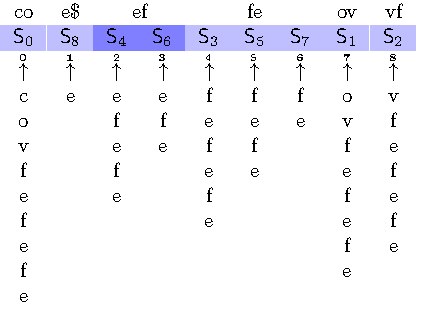
\includegraphics{kapitel/saca_algorithmen/bpr/algorithmus/phase2/buckets_initial_compare/image.pdf}
			\hspace{1em}
			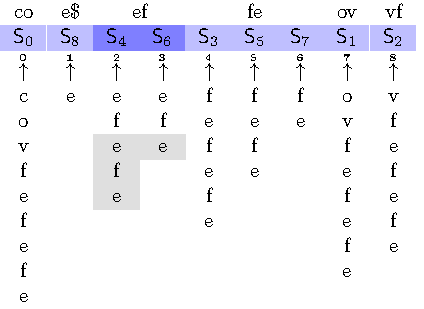
\includegraphics{kapitel/saca_algorithmen/bpr/algorithmus/phase2/buckets_initial_compare_highlight/image.pdf}
	}
	\caption{Vergleich zweier Suffixe innerhalb eines Buckets}
	\label{fig:inner_bucket}
\end{figure}
Am bereits zuvor eingeführten Beispiel beginnen wir, den Bucket \bucket{\textup{ef}} zu sortieren (Abbildung~\ref{fig:inner_bucket}). Der Bucket beinhaltet die Suffixe \suffix{4} und \suffix{6}, welche nach dem Sortierschritt in Phase 1 einen gemeinsamen Präfix der Länge \(d = 2\) haben. Da die Sortierung der Suffixe lexikographisch erfolgen soll, können gemeinsame Präfixe ignoriert werden, ohne die Korrektheit der Sortierung zu beeinflussen. 
\begin{lemma}[Gemeinsamer Präfix]
	\label{lemma:common_prefix}
	\normalfont
    Haben zwei Suffixe \suffix{i} und \suffix{j} einen gemeinsamen Präfix der Länge \offset, so ist \(\suffix{i} \leq \suffix{j}\) genau dann, wenn \(\suffix{i+\offset} \leq \suffix{j+\offset}\). Dies folgt direkt aus der Definition der lexikographischen Ordnung.
\end{lemma}
Für Suffixe \(\suffix{i}, \suffix{j}\) mit \(i, j \in \mathsf{b}\) gibt der Level des Buckets \(\mathsf{b}\) eine untere Schranke für \offset an. Im Falle des Beispiels genügt es also, die Suffixe \(\suffix{4+2} = \suffix{6}\) und \(\suffix{6+2} = \suffix{8}\) zu vergleichen (Abbildung~\ref{fig:buckets_compare_and_sort}, oben links). Da selbstverständlich Suffixe der Suffixe von \inputtext auch selbst Suffixe von \inputtext sind, befinden sich auch diese in \sa. Falls  sich \(\suffix{i+\offset}\) und \(\suffix{j+\offset}\) bereits in verschiedenen Buckets befinden, ist das lexikographische Verhältnis dieser beiden Suffixe bereits bekannt. Um dies herauszufinden, werden die Bucket Pointer der entsprechenden Suffixe verglichen. Diese befinden sich im Array \bptr, welches bereits in Phase 1 initialisiert wurde und beinhalten einen Verweis auf die rechte Grenze des Buckets, in dem sich der jeweilige Suffix befindet.\par
\begin{figure}[ht]
	\resizebox{\textwidth}{!}{
		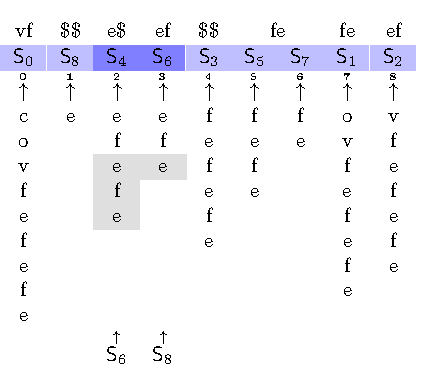
\includegraphics[valign=t]{kapitel/saca_algorithmen/bpr/algorithmus/phase2/buckets_initial_compare_highlight_label/image.pdf}
		\hspace{1em}
		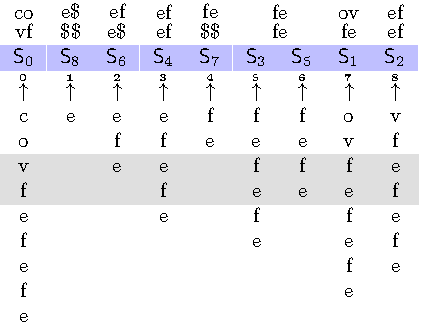
\includegraphics[valign=t]{kapitel/saca_algorithmen/bpr/algorithmus/phase2/buckets_updated/image.pdf}
	}\vspace{1ex}
	\resizebox{\textwidth}{!}{
		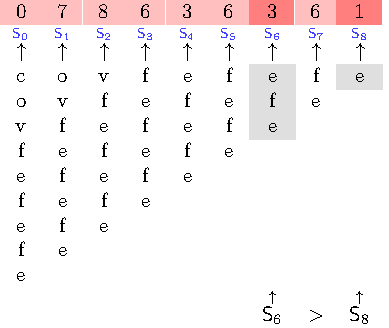
\includegraphics[valign=t]{kapitel/saca_algorithmen/bpr/algorithmus/phase2/bptr_initial_highlighted/image.pdf}
		\hspace{1em}
		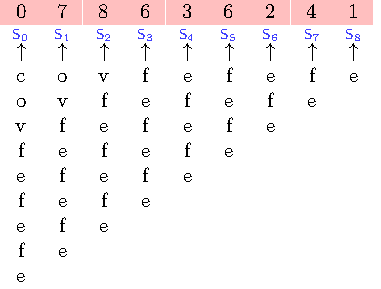
\includegraphics[valign=t]{kapitel/saca_algorithmen/bpr/algorithmus/phase2/bptr_updated/image.pdf}
	}
	\caption[Buckets sowie Bucket-Pointer vor und nach der ersten Verfeinerung]{Buckets (oben) sowie Bucket-Pointer (unten) vor und nach der ersten Verfeinerung. Es ist gut zu erkennen, dass bereits bei einer Rekursionstiefe von 1 nur noch ein nicht eindeutig sortierter Bucket existiert.}
	\label{fig:buckets_compare_and_sort}
\end{figure}
Abbildung~\ref{fig:buckets_compare_and_sort} (unten links) zeigt die Bucket Pointer der Suffixe \(\suffix{6}\) (Bucket \(\bucket{\textup{ef}}\) mit rechter Grenze an Index 3 in \sa) und \(\suffix{8}\) (Bucket \(\bucket{\textup{e\$}}\) mit rechter Grenze an Index 1 in \sa). Aus einem einfachen Vergleich dieser Bucket Pointer geht hervor, dass \(\suffix{8}\) lexikographisch kleiner ist als \(\suffix{6}\). Mithilfe von Lemma \ref{lemma:common_prefix} kann daraus geschlossen werden, dass auch \(\suffix{6}\) lexikographisch kleiner ist als \(\suffix{4}\). Ein solcher Vergleich kann durch zwei Zugriffe auf das Array \bptr in konstanter Zeit durchgeführt werden. Zur Veranschaulichung zeigt Abbildung~\ref{fig:buckets_compare_and_sort} (rechts) den Zustand von \sa und \bptr, wenn in \sa nur noch Level-4-Buckets enthalten sind. Nachdem ein Verfeinerungsschritt in einem Bucket \(\bucket{\textup{p}} = [l,r]\) in kleinere Buckets durchgeführt wurde, müssen außerdem die zugehörigen Bucket-Pointer im Array \bptr angepasst werden. Dazu wird der Bucket \(\bucket{\textup{p}}\) von rechts nach links durchlaufen, wobei für jeden darin enthaltenen Suffix \(\sa[i], l \leq i \leq r,\) der Sortiertschlüssel \(\bptr[\sa[i]+\offset]\) abgefragt. Es wird dann zwischen zwei Fällen unterschieden:

\begin{description}
	\item[Fall 1:]\(\bptr[\sa[i-1]+\offset] = \bptr[\sa[i]+\offset]\) \\
		Die Sortierschlüssel der Suffixe \(\sa[i-1]\) und \(\sa[i]\) sind identisch. Daher konnte in diesem Schritt keine echte Sortierung dieser beiden Suffixe vorgenommen werden. Deshalb befinden sie sich nach wie vor in einem gemeinsamen Bucket und \(\bptr[\sa[i-1]]\) wird auf \(\bptr[\sa[i]]\) gesetzt.
	\item[Fall 2:] \(\bptr[\sa[i-1]+\offset] \neq \bptr[\sa[i]+\offset]\) \\
		Die Sortierschlüssel der Suffixe \(\sa[i-1]\) und \(\sa[i]\) unterscheiden sich. Die Suffixe konnten also sortiert werden und befinden sich nach der Verfeinerung in unterschiedlichen Buckets. \(\sa[i-1]\) ist das erste Element von rechts in dem neu beginnenden Bucket. Folglich wird \(\bptr[\sa[i-1]]\) auf \(i-1\) gesetzt.
\end{description}

\noindent Nachdem die Bucket-Pointer aktualisiert wurden, ist der Sortiervorgang für \(\bucket{\textup{p}}\) abgeschlossen und es kann rekursiv fortgefahren werden. Das fertig sortierte Suffix-Array (links), welches nach Abschluss der Sortierung nur noch Buckets der Größe 1 enthält, sowie die dazugehörigen Bucket-Pointer (rechts) sind in Abbildung~\ref{fig:buckets_final} zu sehen.\par\smallskip
\begin{figure}[ht]
	\resizebox{\textwidth}{!}{
		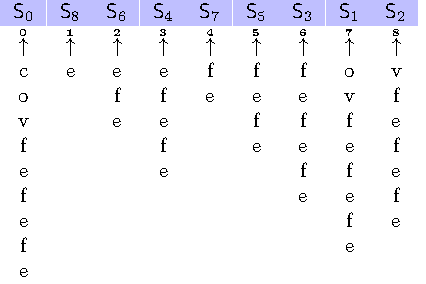
\includegraphics{kapitel/saca_algorithmen/bpr/algorithmus/phase2/buckets_final/image.pdf}
		\hspace{1em}
		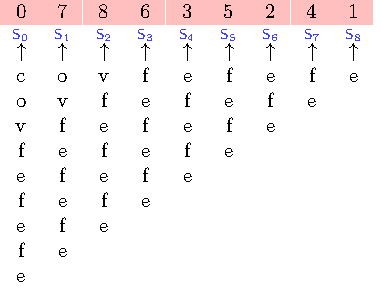
\includegraphics{kapitel/saca_algorithmen/bpr/algorithmus/phase2/bptr_final/image.pdf}
	}
	\caption[Sortiertes Suffix-Array und zugehörige Bucket-Pointer]{Sortiertes Suffix-Array (links) und zugehörige Bucket-Pointer (rechts)}
	\label{fig:buckets_final}
\end{figure}
Bei der Wahl des Sortierverfahrens unterscheidet \bpr abhängig von der Größe eines Buckets zwischen \emph{Insertionsort} und \emph{Quicksort}. Für Buckets mit maximal 15 Elementen wird \emph{Insertionsort} verwendet, während alle größeren Buckets mit einer Variante von \emph{Quicksort} sortiert werden. Ergänzend zur Partitionierung des Buckets in zwei Hälften werden alle an das Pivotelement angrenzenden Elemente mit gleichem Sortierschlüssel von den rekursiv zu sortierenden Partitionen ausgenommen, solange bis in beide Richtungen das erste Element mit unterschiedlichem Schlüssel gefunden wird. Diese Heuristik sorgt dafür, dass je nach Struktur des Eingabestrings die zu sortierenden Partitionen deutlich verkleinert werden können, falls in einem Bucket viele Suffixe den gleichen Schlüssel haben.\par\smallskip
Falls es aufgrund der Struktur des Eingabestrings vorkommt, dass innerhalb eines Buckets alle Suffixe einen gemeinsamen Präfix einer deutlich größeren Länge als \offset haben, dann würde \emph{Quicksort} (bzw. bei kleinen Buckets \emph{Insertionsort}) für mehrere Schritte in der Rekursion versuchen, ausschließlich Elemente mit gleichem Schlüssel zu sortierten. Dies beeinflusst zwar nicht die Korrektheit des Verfahrens, allerdings entsteht durch jeden überflüssigen Sortiervorgang ein unerwünschter und vermeidbarer Aufwand. Um dem entgegen zu wirken, wird eine Heuristik verwendet, welche nach einem \glqq erfolglosen\grqq{} Sortiervorgang die Länge des längsten gemeinsamen Präfixes aller Suffixe in diesem Bucket bestimmt. Der darauf folgende Rekursionsschritt wird dann mit dieser Länge anstelle von \offset aufgerufen.

\subsubsection{Beispiel}
\label{bpr:algorithmus:beispiel}

\newcolumntype{M}[1]{>{\centering\arraybackslash}m{#1}}
\newcommand{\mc}[2]{\multicolumn{#1}{c}{#2}}

Am Beispiel \texttt{caabaccaabacaa} wird noch einmal die Funktionsweise des gesamten Algorithmus im Detail demonstriert. Das Beispiel dient der Übersichtlichkeit und Vergleichbarkeit zu anderen Algorithmen.
\begin{figure}[ht]
    {\centering\begin{minipage}{\textwidth}
        {\large \textsc{Schritt 1}} \hfill {\Large \textsc{Phase 1}}\par\medskip
        \resizebox{\textwidth}{!}{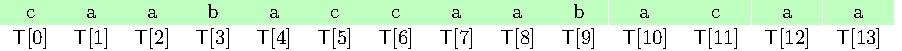
\includegraphics{kapitel/saca_algorithmen/bpr/algorithmus/beispiel/phase_1/step_01/t/image.pdf}}\par\medskip
        \resizebox{\textwidth}{!}{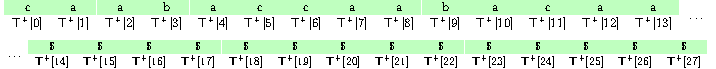
\includegraphics{kapitel/saca_algorithmen/bpr/algorithmus/beispiel/phase_1/step_01/tplus/image.pdf}}\\
    \end{minipage}}
    \caption[\bpr: Phase 1, Schritt 1]{\bpr: Phase 1, Schritt 1. Oben: Eingabetext \inputtext. Unten: Erweiterter Eingabetext \inputtextplus.}
    \label{bpr:p1s1}
\end{figure}
Der erste Schritt besteht lediglich daraus, die Eingabe aufzubereiten, indem \(n\) symbolische Sentinels an das Eingabewort angehängt werden. Dieses Vorgehen wird im Paper beschrieben, im Algorithmus allerdings aufgrund des linearen Speicherbedarfs nicht direkt umgesetzt. \par
\begin{figure}[ht]
    {\centering\begin{minipage}{\textwidth}
        {\large \textsc{Schritt 2}}\par\medskip
        \resizebox{\textwidth}{!}{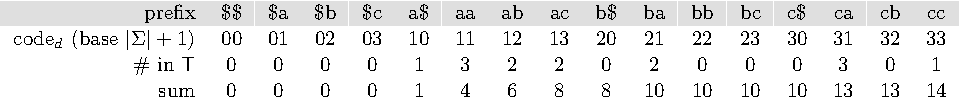
\includegraphics{kapitel/saca_algorithmen/bpr/algorithmus/beispiel/phase_1/step_02/bkt/image.pdf}}\par\medskip
        \resizebox{\textwidth}{!}{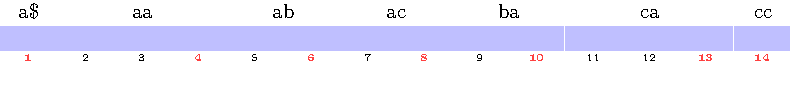
\includegraphics{kapitel/saca_algorithmen/bpr/algorithmus/beispiel/phase_1/step_02/buckets/image.pdf}}
    \end{minipage}}
    \caption[\bpr: Phase 1, Schritt 2]{\bpr: Phase 1, Schritt 2. Oben: Größen und Positionen der Buckets. Unten: Leere Buckets im Suffixarray.}
    \label{bpr:p1s2}
\end{figure}
Im zweiten Schritt wird der Bucketsort Algorithmus (\cref{section:bucketsort}, Seite \pageref{section:bucketsort}) durchgeführt, um eine Vorsortierung für das Suffixarray zu erlangen. Die Tiefe, die für Bucketsort als Parameter verwendet wird, leitet sich in festgelegten Stufen aus der Größe des Alphabets ab und beträgt auch für große Alphabete mindestens 3. In diesem Beispiel wird aus Gründen der Übersichtlichkeit nur eine Tiefe von 2 verwendet.\par
\begin{figure}[ht]
    {\centering\begin{minipage}{\textwidth}
        {\large \textsc{Schritt 3}}\par\medskip
        \resizebox{.56\textwidth}{!}{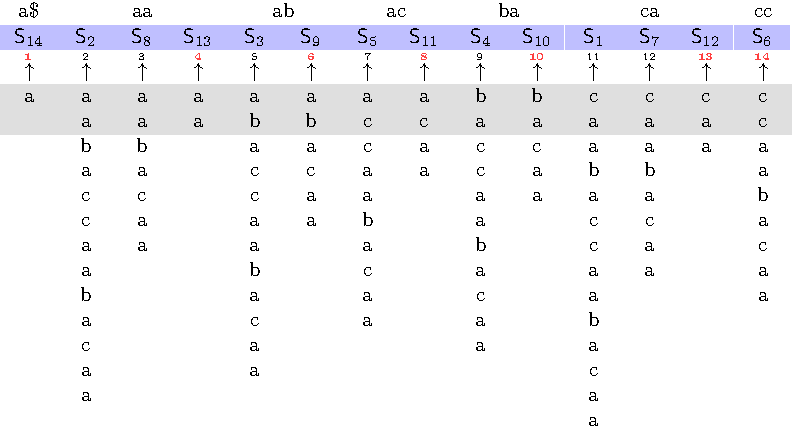
\includegraphics{kapitel/saca_algorithmen/bpr/algorithmus/beispiel/phase_1/step_03/buckets/image.pdf}}
        \hfill
        \resizebox{.4\textwidth}{!}{\includegraphics{kapitel/saca_algorithmen/bpr/algorithmus/beispiel/phase_1/step_03/bptr/image.pdf}}
    \end{minipage}}
    \caption[\bpr: Phase 1, Schritt 3]{\bpr: Phase 1, Schritt 3. Links: Befüllte Buckets im Suffixarray. Rechts Initiales \bptr-Array.}
    \label{bpr:p1s3}
\end{figure}
Zu Beginn des dritten Schrittes sind die rechten Grenzen der Buckets bereits bekannt (siehe \cref{bpr:p1s2}, rot markiert) und die Suffixe in die entsprechenden Buckets einsortiert. Daraus wird im Anschluss das Bucket-Pointer Array (\cref{bpr:p1s2}, rechts)  berechnet, in dem für jeden Suffix gespeichert ist, in welchem Bucket sich dieser in der aktuellen Sortierung befindet. Die Buckets werden dabei über ihre rechte inklusive Grenze identifiziert.
\begin{figure}[H]
    {\centering\begin{minipage}{\textwidth}
        {\large \textsc{Schritt 1}} \hfill {\Large \textsc{Phase 2}}\par\medskip
        \resizebox{.56\textwidth}{!}{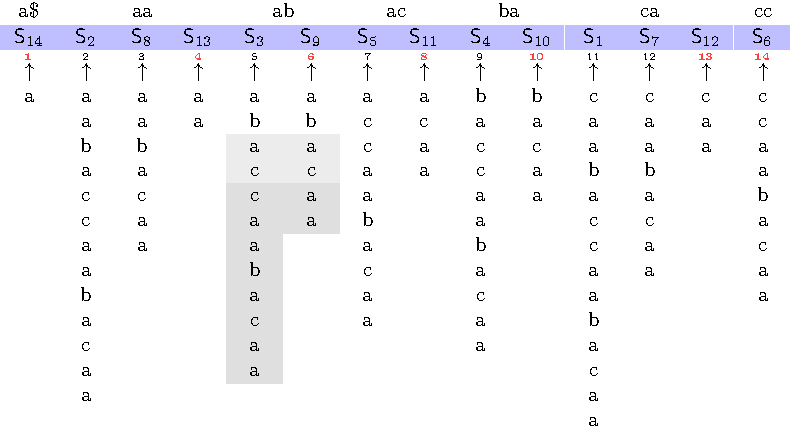
\includegraphics{kapitel/saca_algorithmen/bpr/algorithmus/beispiel/phase_2/step_01/buckets_before/image.pdf}}
        \hfill
        \resizebox{.4\textwidth}{!}{\includegraphics{kapitel/saca_algorithmen/bpr/algorithmus/beispiel/phase_2/step_01/bptr_before/image.pdf}}\\
        \resizebox{.56\textwidth}{!}{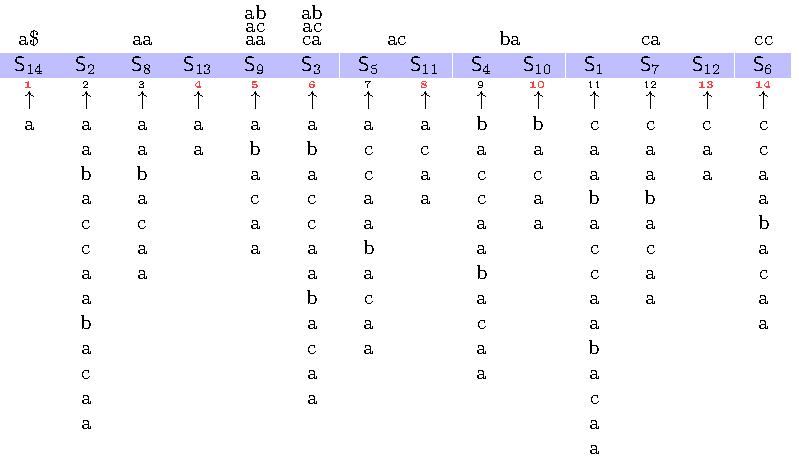
\includegraphics{kapitel/saca_algorithmen/bpr/algorithmus/beispiel/phase_2/step_01/buckets_after/image.pdf}}
        \hfill
        \resizebox{.4\textwidth}{!}{\includegraphics{kapitel/saca_algorithmen/bpr/algorithmus/beispiel/phase_2/step_01/bptr_after/image.pdf}}
    \end{minipage}}
    \caption[\bpr: Phase 2, Schritt 1]{\bpr: Phase 2, Schritt 1. Oben: \sa und \bptr vor dem Sortierschritt. Unten: \sa und \bptr nach dem Sortierschritt.}
    \label{bpr:p2s1}
\end{figure}
Sobald die Bucket-Pointer bestimmt sind, ist ein Zustand erreicht, von dem aus im Anschluss in der zweiten Phase alle Buckets Schritt für Schritt verfeinert werden können. Diese Verfeinerung erfolgt iterativ über die Buckets und rekursiv innerhalb der Buckets. Die Reihenfolge, in der die nach Phase 1 entstandenen Buckets sortiert werden, ist im Grundalgorithmus für die Korrektheit irrelevant. Unter Verwendung der Copy-Technik lässt sich der Rechenaufwand aber durch eine geschickte Wahl der Reihenfolge verringern.\par
Die Verfeinerung erfolgt innerhalb eines Buckets Schrittweise mit einer Schrittgröße, die der zuvor gewählten Tiefe von Bucketsort entspricht. In diesem Beispiel wird zuerst der Bucket \bucket{ab} verfeinert. Aus der Bucket-Pointer Tabelle lässt sich nach einem Rekursionsschritt ablesen, dass die beiden darin enthaltenen Suffixe in ihrer Reihenfolge vertauscht werden müssen. Danach ist der Bucket fertig sortiert und die Bucket-Pointer werden an die neue Sortierung angepasst.\par
Anschließend wird der Bucket \bucket{ac} sortiert (\cref{bpr:p2s2}), dessen Suffixe sich bereits nach einem gemeinsamen Präfix der Länge 2 unterscheiden. Aus der Bucket-Pointer Tabelle kann damit direkt abgelesen werden, in welchen Buckets sich die korrespondierenden Suffixe befinden, woraus dann die Reihenfolge abgeleitet wird. Das Vertauschen von \(\suffix{5}\) und \(\suffix{11}\) führt zur richtigen Reihenfolge.\par
Die darauf folgende Sortierung des Buckets \bucket{ba} erfolgt analog (\cref{bpr:p2s34}, oben).
Zuletzt werden in den Schritten 4 und 5 (\cref{bpr:p2s34}, unten und \cref{bpr:p2s5}) die Buckets \bucket{aa} und \bucket{ca} sortiert. Beide bestehen aus jeweils drei Suffixen, die sich alle bereits eindeutig anhand der Positionen in der nebenstehenden Tabelle in Buckets der Größe 1 einsortieren lassen. Nach Schritt 5 existieren schließlich nur noch Buckets der Größe 1 und das Suffixarray ist damit fertig sortiert. An dieser Stelle verwirft der Algorithmus das Array \bptr und gibt \sa als Lösung aus.
\begin{figure}[H]
    {\centering\begin{minipage}{\textwidth}
        {\large \textsc{Schritt 2}}\par\medskip
        \resizebox{.56\textwidth}{!}{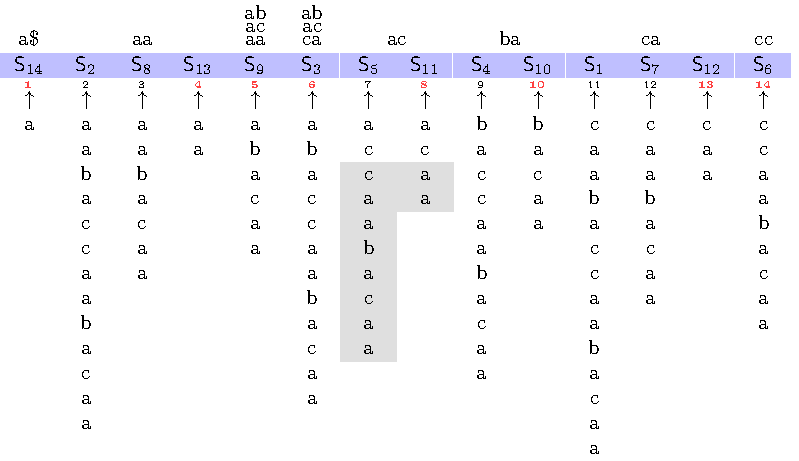
\includegraphics{kapitel/saca_algorithmen/bpr/algorithmus/beispiel/phase_2/step_02/buckets_before/image.pdf}}
        \hfill
        \resizebox{.4\textwidth}{!}{\includegraphics{kapitel/saca_algorithmen/bpr/algorithmus/beispiel/phase_2/step_02/bptr_before/image.pdf}}\\
        \resizebox{.56\textwidth}{!}{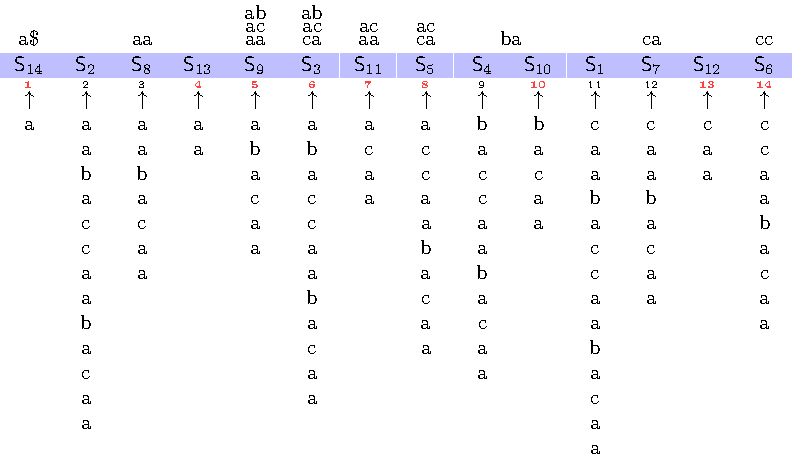
\includegraphics{kapitel/saca_algorithmen/bpr/algorithmus/beispiel/phase_2/step_02/buckets_after/image.pdf}}
        \hfill
        \resizebox{.4\textwidth}{!}{\includegraphics{kapitel/saca_algorithmen/bpr/algorithmus/beispiel/phase_2/step_02/bptr_after/image.pdf}}\\
    \end{minipage}}
    \caption[\bpr: Phase 2, Schritt 2]{\bpr: Phase 2, Schritt 2. Oben: \sa und \bptr vor dem Sortierschritt. Unten: \sa und \bptr nach dem Sortierschritt.}
    \label{bpr:p2s2}
\end{figure}
\begin{figure}[H]
    {\centering\begin{minipage}{\textwidth}
        {\large \textsc{Schritt 3}}\par\medskip
        \resizebox{.56\textwidth}{!}{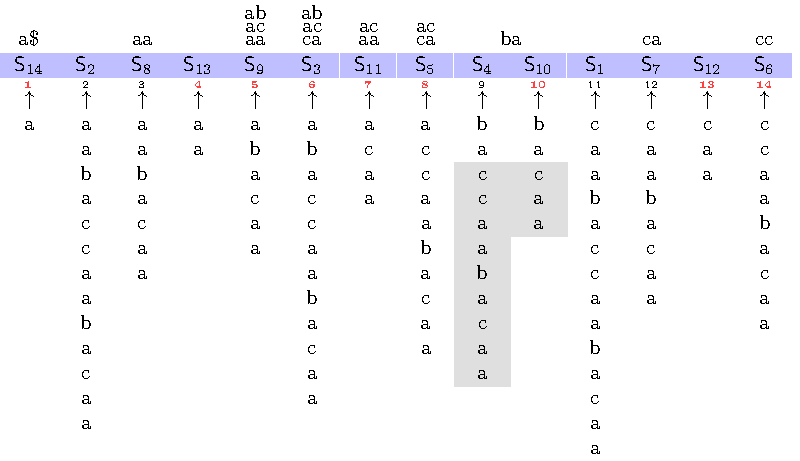
\includegraphics{kapitel/saca_algorithmen/bpr/algorithmus/beispiel/phase_2/step_03/buckets_before/image.pdf}}
        \hfill
        \resizebox{.4\textwidth}{!}{\includegraphics{kapitel/saca_algorithmen/bpr/algorithmus/beispiel/phase_2/step_03/bptr_before/image.pdf}}\\
        \resizebox{.56\textwidth}{!}{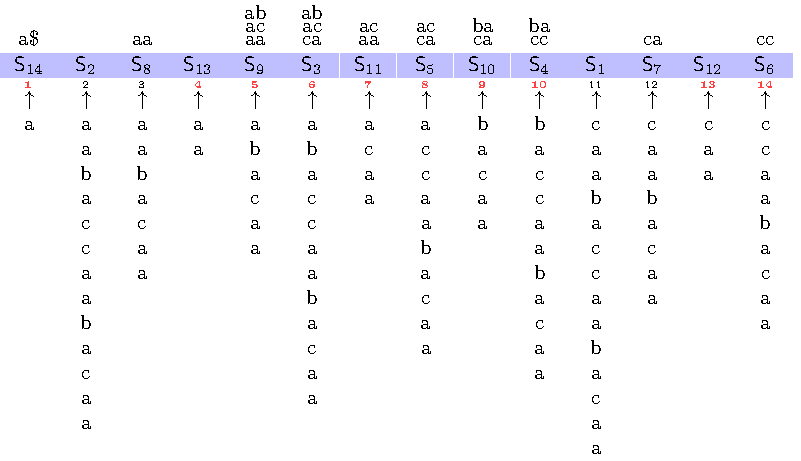
\includegraphics{kapitel/saca_algorithmen/bpr/algorithmus/beispiel/phase_2/step_03/buckets_after/image.pdf}}
        \hfill
        \resizebox{.4\textwidth}{!}{\includegraphics{kapitel/saca_algorithmen/bpr/algorithmus/beispiel/phase_2/step_03/bptr_after/image.pdf}}\\
        \par
        {\large \textsc{Schritt 4}}\par\medskip
        \resizebox{.56\textwidth}{!}{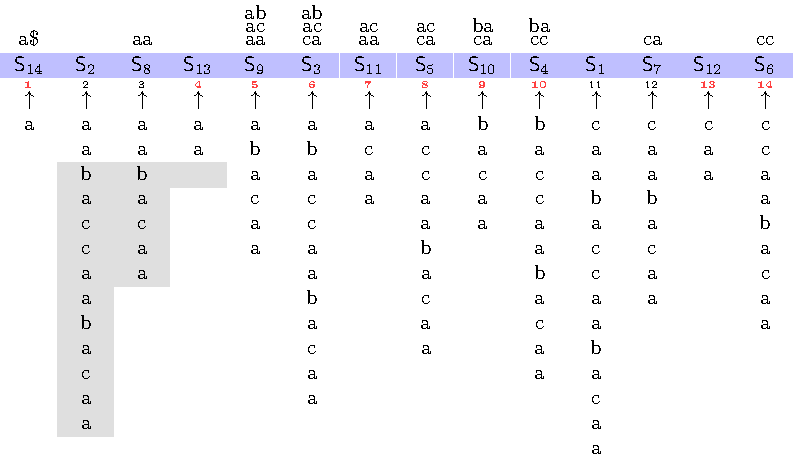
\includegraphics{kapitel/saca_algorithmen/bpr/algorithmus/beispiel/phase_2/step_04/buckets_before/image.pdf}}
        \hfill
        \resizebox{.4\textwidth}{!}{\includegraphics{kapitel/saca_algorithmen/bpr/algorithmus/beispiel/phase_2/step_04/bptr_before/image.pdf}}\\
        \resizebox{.56\textwidth}{!}{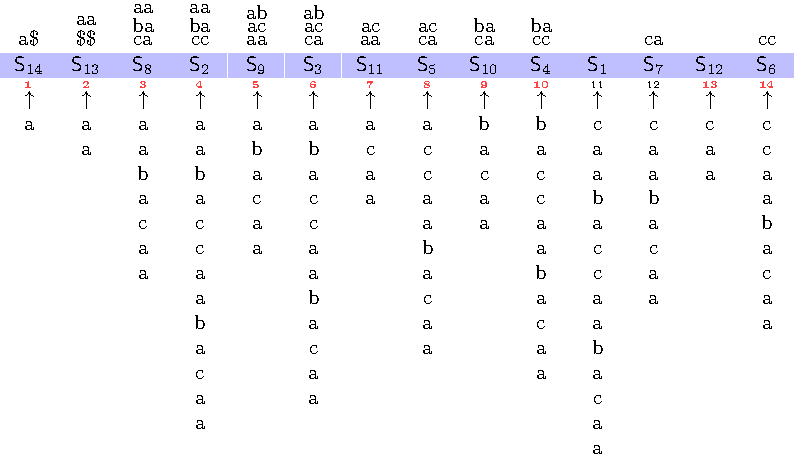
\includegraphics{kapitel/saca_algorithmen/bpr/algorithmus/beispiel/phase_2/step_04/buckets_after/image.pdf}}
        \hfill
        \resizebox{.4\textwidth}{!}{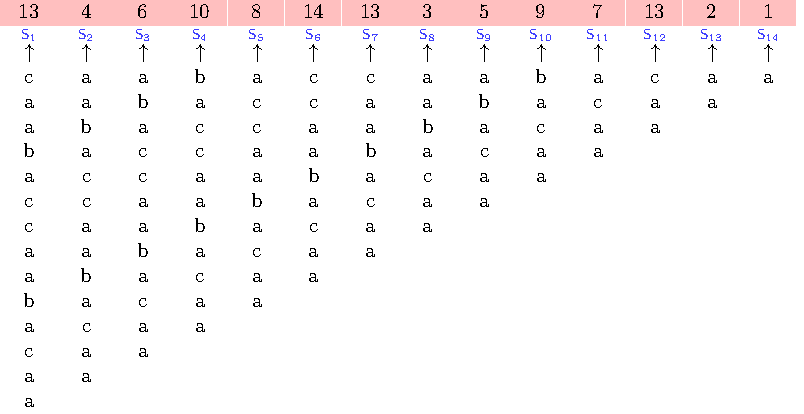
\includegraphics{kapitel/saca_algorithmen/bpr/algorithmus/beispiel/phase_2/step_04/bptr_after/image.pdf}}\\
    \end{minipage}}
    \caption[\bpr: Phase 2, Schritte 3 und 4]{\bpr: Phase 2, Schritte 3 und 4. Jeweils oben: \sa und \bptr vor dem Sortierschritt. Jeweils unten: \sa und \bptr nach dem Sortierschritt.}
    \label{bpr:p2s34}
\end{figure}
\begin{figure}[H]
    {\centering\begin{minipage}{\textwidth}
        {\large \textsc{Schritt 5}}\par\medskip
        \resizebox{.56\textwidth}{!}{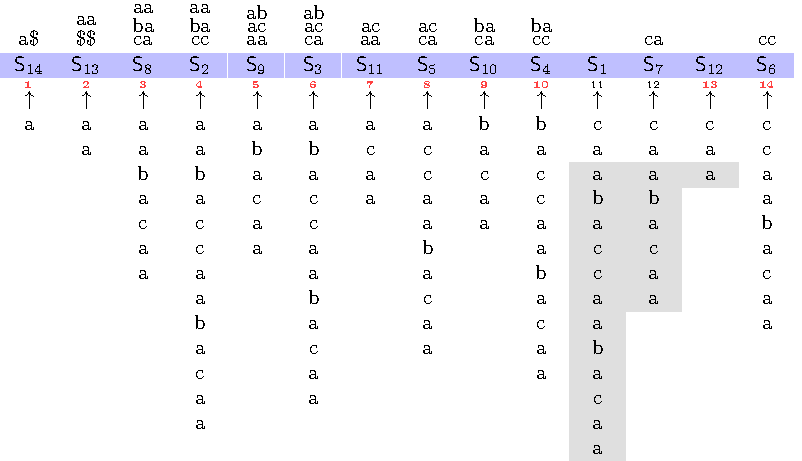
\includegraphics{kapitel/saca_algorithmen/bpr/algorithmus/beispiel/phase_2/step_05/buckets_before/image.pdf}}
        \hfill
        \resizebox{.4\textwidth}{!}{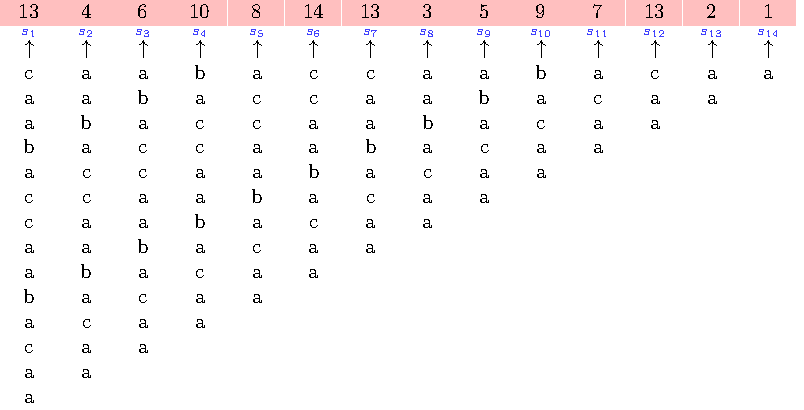
\includegraphics{kapitel/saca_algorithmen/bpr/algorithmus/beispiel/phase_2/step_05/bptr_before/image.pdf}}\\
        \resizebox{.56\textwidth}{!}{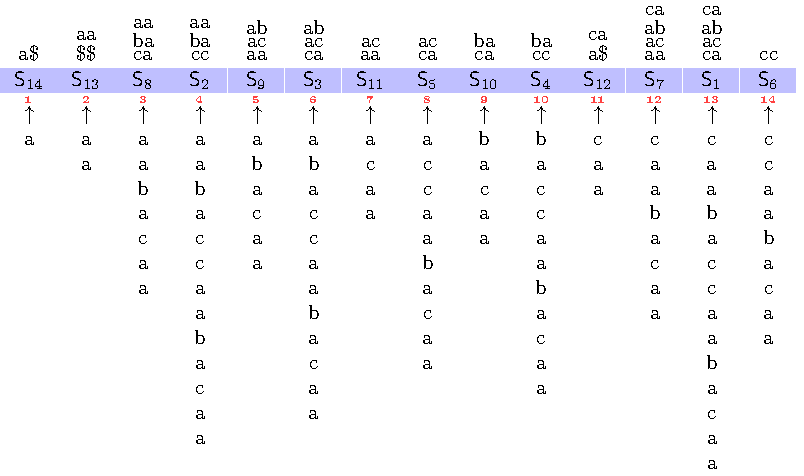
\includegraphics{kapitel/saca_algorithmen/bpr/algorithmus/beispiel/phase_2/step_05/buckets_after/image.pdf}}
        \hfill
        \resizebox{.4\textwidth}{!}{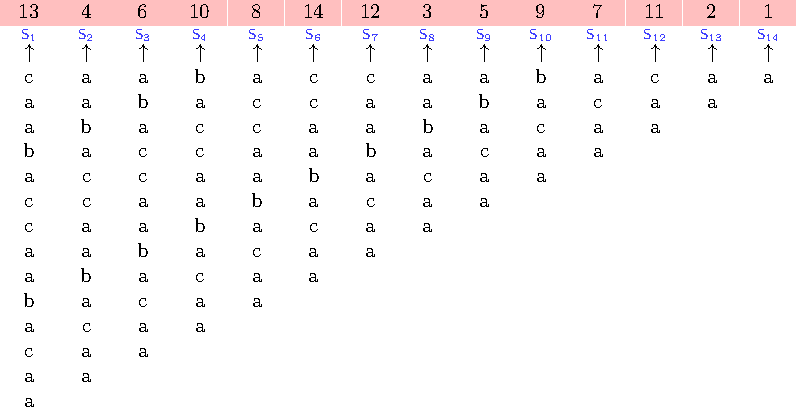
\includegraphics{kapitel/saca_algorithmen/bpr/algorithmus/beispiel/phase_2/step_05/bptr_after/image.pdf}}\\
    \end{minipage}}
    \caption[\bpr: Phase 2, Schritt 5]{\bpr: Phase 2, Schritt 5. Oben: \sa und \bptr vor dem Sortierschritt. Unten: \sa und \bptr nach dem Sortierschritt.}
    \label{bpr:p2s5}
\end{figure}

